%!TEX spellcheck = es_ES
\documentclass[12pt,a4paper,addpoints,answers]{exam}
%\documentclass[12pt,a4paper,addpoints]{exam}
\usepackage[utf8]{inputenc}
\usepackage[spanish]{babel}
\usepackage{adjustbox}
\usepackage{multirow}
\usepackage{graphicx}
\usepackage{tikz}
\usepackage{amsmath}
\usepackage{setspace}
\usepackage{afterpage}
\usepackage{ulem}

% Entidad-relación con TIKZ
\usetikzlibrary{er,shapes,positioning,calc}
\newcommand{\key}[1]{\underline{#1}}

\tikzset{weak entity/.style={entity ,double  distance =2pt}}
\tikzset{weak relationship/.style={relationship, double distance =2pt}}
\tikzset{
    -|/.style={to path={-| (\tikztotarget)}},
    |-/.style={to path={|- (\tikztotarget)}},
}

% Términos en castellano
\pointpoints{Punto}{Puntos}
\bonuspointpoints{Punto extra}{Puntos extra}
\renewcommand{\solutiontitle}{\noindent\textbf{Solución propuesta:}\enspace\\}
\chqword{Pregunta}
\chpgword{Página}
\chpword{Punto}
\chbpword{Punto extra}
\chsword{Obtenidos}
\chtword{Totales}
\hpword{Puntos:}
\hsword{Nota:}
\hqword{Ejercicio:}
\htword{Total:}

\pagestyle{headandfoot}
\firstpageheadrule
\runningheadrule
\firstpageheader{Bases de Datos I}{}{Primer parcial\\Curso 2021/2022}
\runningheader{Bases de Datos I}{}{Primer parcial\\Curso 2021/2022}
\firstpagefooter{}{}{\thepage\,/\,\numpages}
\runningfooter{}{}{\thepage\,/\,\numpages}

\begin{document}
\begin{center}
{\Huge Bases de Datos I -- Primer parcial}\\
\vspace{2em}
{\Large Modelo Entidad-Relación y Modelo Relacional}\\
\vspace{1em}
31 de marzo de 2022
\end{center}

\begin{center}\textbf{Normativa de examen}\end{center}
\begin{itemize}
    \item No está permitido el uso de dispositivos móviles ni otros dispositivos electrónicos, así como libros ni apuntes.
    \item Durante el examen, los profesores podrán solicitar acreditar la identidad de los participantes en el mismo. Deberá tener en todo momento su Documento Nacional de Identidad y/o Carné de la UPM visible sobre la mesa.
    \item Deberá escribir su nombre y firma, \textbf{con bolígrafo}, en todas las hojas de las que consta el examen.
    \item El examen se resolverá \textbf{obligatoriamente a bolígrafo}.
    \item No se permite abandonar el aula de examen durante los \textbf{primeros 15 minutos}. Transcurrido este tiempo, no se permitirá entrar al examen.
    \item Este examen consta de \numquestions\ ejercicios para un total de \numpoints\ puntos.
    \item El examen tiene una duración máxima de \textbf{1.5 horas}.
    \item Justifique sus respuestas lo mejor posible indicando, si fuese necesario, los pasos realizados.
    \item La fecha para la revisión del examen se anunciará en el Moodle de la asignatura.
    \item Según recoge la guía de la asignatura, es necesario obtener 4 puntos sobre 10 (2 sobre 5) en cada bloque para aprobar la asignatura por evaluación continua.
\end{itemize}

\begin{questions}
  \titledquestion{Entidad-Relación y paso a tablas}
  \label{question:entidad-relacion}
  (\totalpoints\ puntos) \textbf{\large\thequestiontitle}

  \begin{parts}
  \part[3\half] \textbf{Modelado conceptual}: Un grupo de investigación está desarrollando un sistema de análisis de redes sociales para extraer conocimiento de las relaciones personales entre seres humanos. En una primera fase han identificado la necesidad de diseñar una base de datos para almacenar la información obtenida de una conocida red social.

  El núcleo principal de la red social son sus usuarios y, por supuesto, los mensajes que publican. La API de la red social nos permite obtener el identificador numérico de cada usuario, así como su nombre de usuario, su descripción, la fecha en la que se registró y si tiene o no foto de perfil. Con respecto a los mensajes que se publican en la red social, es posible acceder al identificador único del mismo así como al contenido del mensaje y la fecha de publicación. Obviamente, hay que conocer qué usuario ha publicado qué mensajes, sabiendo que cada mensaje solo tiene un autor. En esta red social es posible responder a un mensaje con otro, por lo que es importante para los análisis posteriores llevar un registro de qué mensaje es una respuesta a otro.

  Por otro lado, el sistema utilizará un modelo automatizado de clasificación de los mensajes mediante etiquetas. Estas etiquetas se identifican por su nombre, aunque también es necesario conocer su descripción y la fecha de creación. Es importante destacar que las etiquetas no son excluyentes, por lo que es posible asignar múltiples etiquetas a un mismo mensaje.

  \textbf{Se pide}: realizar el modelado conceptual de la base de datos descrita anteriormente mediante el diagrama Entidad-Relación, incluyendo los dominios de aquellos atributos que no sean un tipo simple. Se penalizará la inclusión de elementos no necesarios o redundantes.

  \begin{solutionorbox}
    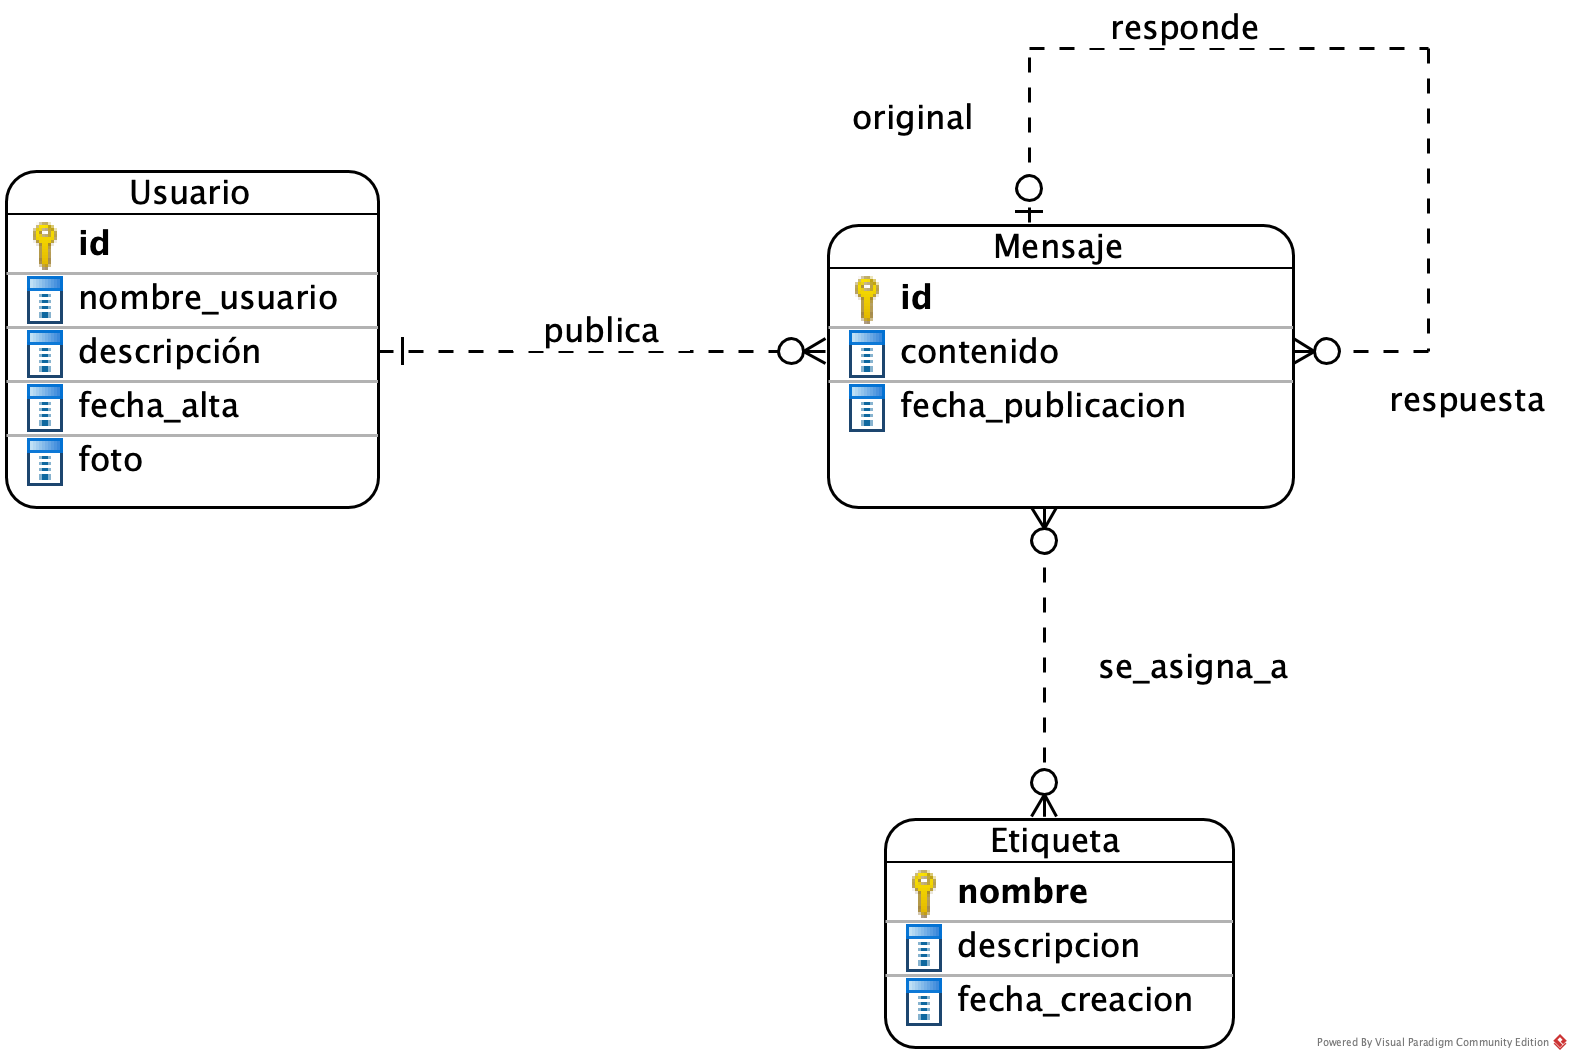
\includegraphics[width=0.9\textwidth]{SNA.png}
  \end{solutionorbox}
  \vspace{3em}

  \newpage
  \part[1\half] \textbf{Paso a tablas}: Dado el siguiente modelo Entidad-Relación realiza el paso a tablas para obtener el modelo relacional correspondiente:
  \begin{figure}[h]
  \centering
  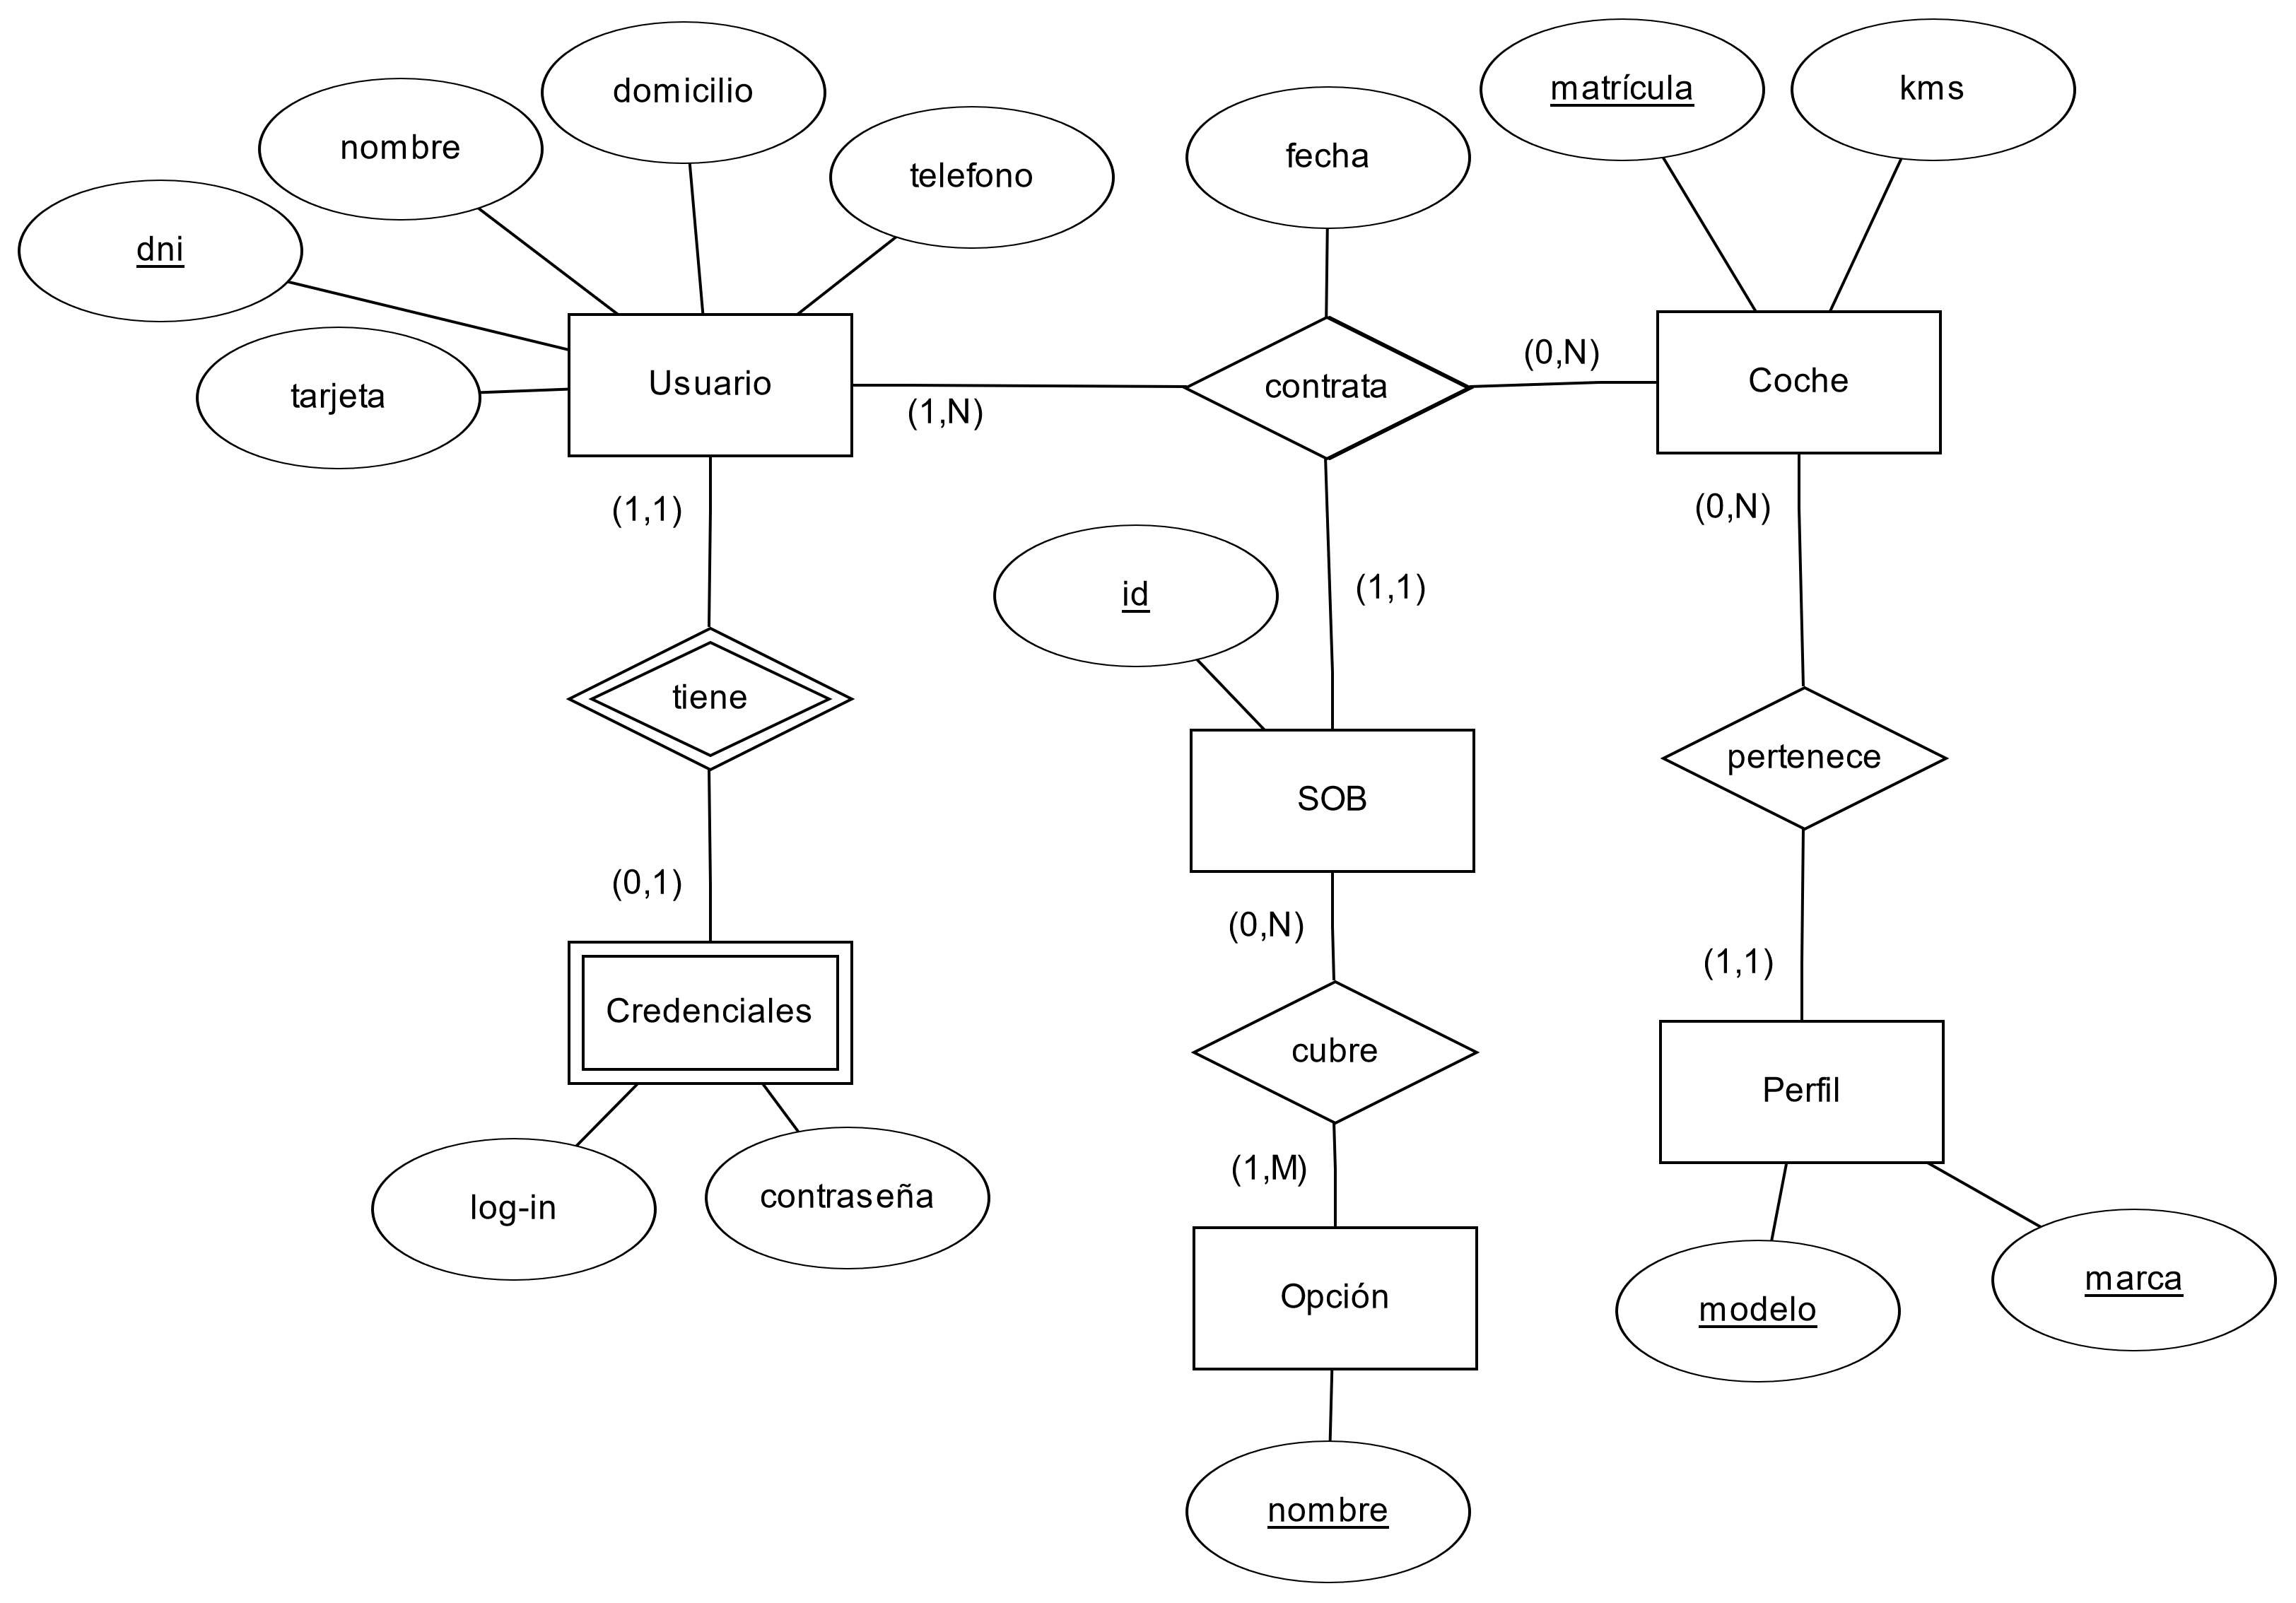
\includegraphics[width=\textwidth]{ejercicio-8.png}
  \end{figure}
  
  \begin{solutionorbox}
  \begin{adjustbox}{max height=0.75\textheight}
      \begin{tikzpicture}[relation/.style={rectangle split, rectangle split parts=#1, rectangle split part align=base, draw, anchor=center, align=center, text height=3mm, text centered}]\hspace*{-0.3cm}
      \node (credencialestitle) {\textbf{Credenciales}};
      \node [relation=3, rectangle split horizontal, anchor=west, right=0.1cm of credencialestitle.east, anchor=west] (credenciales)
        {\underline{dni}%
        \nodepart{two}   \dashuline{log-in}
        \nodepart{three} contraseña};
      
      \node [anchor=north west,below=1.5cm of credencialestitle.west, anchor=north west] (usuariotitle) {\textbf{Usuario}};
      \node [relation=5, rectangle split horizontal, anchor=west, right=0.1cm of usuariotitle.east, anchor=west] (usuario)
        {\underline{dni}%
         \nodepart{two}   tarjeta
         \nodepart{three} nombre
         \nodepart{four}  domicilio
         \nodepart{five}  teléfono};
    
      \node [anchor=north west,below=1.5cm of usuariotitle.west, anchor=north west] (contratatitle) {\textbf{contrata}};
      \node [relation=4, rectangle split horizontal, anchor=west, right=0.1cm of contratatitle.east, anchor=west] (contrata)
        {\underline{dni}%
         \nodepart{two}   \underline{matrícula}%
         \nodepart{three} \underline{id}%
         \nodepart{four}  \underline{fecha}};
    
      \node [anchor=north west,below=1.5cm of contratatitle.west, anchor=north west] (cochetitle) {\textbf{Coche}};
      \node [relation=4, rectangle split horizontal, anchor=west, right=0.1cm of cochetitle.east, anchor=west] (coche)
        {\underline{matrícula}%
         \nodepart{two}   kms%
         \nodepart{three} modelo%
         \nodepart{four}  marca};
    
      \node [anchor=west, right=1cm of coche.east, anchor=west] (perfiltitle) {\textbf{perfil}};
      \node [relation=2, rectangle split horizontal, anchor=west, right=0.1cm of perfiltitle.east, anchor=west] (perfil)
        {\underline{modelo}%
         \nodepart{two}   \underline{marca}};
    
      \node [anchor=north west,below=1.5cm of cochetitle.west, anchor=north west] (sobtitle) {\textbf{SOB}};
      \node [relation=1, rectangle split horizontal, anchor=west, right=0.1cm of sobtitle.east, anchor=west] (sob)
        {\underline{id}};
      
      \node [anchor=west, right=1cm of sob.east] (cubretitle) {\textbf{cubre}};
      \node [relation=2, rectangle split horizontal, anchor=west, right=0.1cm of cubretitle] (cubre)
      {\underline{id}%
       \nodepart{two} \underline{nombre}};
       
      \node [anchor=west,right=1cm of cubre.east, anchor=west] (opciontitle) {\textbf{Opción}};
      \node [relation=1, rectangle split horizontal, anchor=west, right=0.1cm of opciontitle.east] (opcion)
        {\underline{nombre}};
    
      % CLAVES FORANEAS
        \draw[-latex] (credenciales.one south) -- ++(0,-0.5) -| (usuario.one north);
        \draw[-latex] (contrata.one north) -- ++(0,0.5) -| (usuario.one south);
        \draw[-latex] (contrata.two south) -- ++(0,-0.5) -| (coche.one north);
        \draw[-latex] (contrata.three south) -- ++(0,-0.2) -| ($(coche.four north) + (1,-1)$) -| (sob.one north);
        \draw[-latex] (coche.three north) -- ++(0,0.5) -| (perfil.one north);
        \draw[-latex] (coche.four north) -- ++(0,0.2) -| (perfil.two north);
        \draw[-latex] (cubre.one south) -- ++(0,-0.5) -| (sob.one south);
        \draw[-latex] (cubre.two south) -- ++(0,-0.5) -| (opcion.one south);
      \end{tikzpicture}
  \end{adjustbox}
  \end{solutionorbox}
  \end{parts}
  
  \newpage
  \titledquestion{Modelo relacional}
  \label{question:relacional}
  (\totalpoints\ puntos) \textbf{\large\thequestiontitle}
  
  Utilizando el siguiente modelo relacional resuelva las siguientes consultas usando \textbf{álgebra relacional}:
  
  \vspace{1em}
  \begin{center}
  \begin{adjustbox}{max height=0.35\textheight}
  \begin{tikzpicture}[relation/.style={rectangle split, rectangle split parts=#1, rectangle split part align=base, draw, anchor=center, align=center, text height=3mm, text centered}]\hspace*{-0.3cm}
  \node (alumnotitle) {\textbf{ALUMNO}};
  \node [relation=4, rectangle split horizontal, anchor=west, right=0.5cm of alumnotitle.east, anchor=west] (alumno)
    {\underline{Nmat}%
    \nodepart{two}   Nombre
    \nodepart{three} Apellidos
    \nodepart{four}  Correo};
  
  \node [anchor=north west,below=1.5cm of alumnotitle.west, anchor=north west] (asignaturatitle) {\textbf{ASIGNATURA}};
  \node [relation=4, rectangle split horizontal, anchor=west, right=0.5cm of asignaturatitle.east, anchor=west] (asignatura)
    {\underline{CodA}%
     \nodepart{two}   Nombre
     \nodepart{three} Créditos
     \nodepart{four}  Curso};

  \node [anchor=north west,below=1.5cm of asignaturatitle.west, anchor=north west] (cursatitle) {\textbf{CURSA}};
  \node [relation=4, rectangle split horizontal, anchor=west, right=0.5cm of cursatitle.east, anchor=west] (cursa)
    {\underline{CodA}%
     \nodepart{two}   \underline{Nmat}%
     \nodepart{three} \underline{CodG}%
     \nodepart{four}  \underline{Año}};

  \node [anchor=north west,below=1.5cm of cursatitle.west, anchor=north west] (grupotitle) {\textbf{GRUPO}};
  \node [relation=4, rectangle split horizontal, anchor=west, right=0.5cm of grupotitle.east, anchor=west] (grupo)
    {\underline{CodG}%
     \nodepart{two}   Nombre
     \nodepart{three} Capacidad
     \nodepart{four}  Aula};

  \node [anchor=north west,below=1.5cm of grupotitle.west, anchor=north west] (impartetitle) {\textbf{IMPARTE}};
  \node [relation=4, rectangle split horizontal, anchor=west, right=0.5cm of impartetitle.east, anchor=west] (imparte)
    {\underline{CodP}%
     \nodepart{two}   \underline{CodG}%
     \nodepart{three} \underline{CodA}%
     \nodepart{four}  \underline{Año}};

  \node [anchor=north west,below=1.5cm of impartetitle.west, anchor=north west] (profesortitle) {\textbf{PROFESOR}};
  \node [relation=4, rectangle split horizontal, anchor=west, right=0.5cm of profesortitle.east, anchor=west] (profesor)
    {\underline{CodP}%
     \nodepart{two}   Nombre
     \nodepart{three} Apellidos
     \nodepart{four}  Despacho};

  % CLAVES FORANEAS
  \draw[-latex] (cursa.one north) -- ++(0,0.75) -| ($(asignatura.one south) + (-0.5,0)$);
  \draw[-latex] (cursa.two north) -- ++(0,0.30) -| ($(asignatura.four north) + (1,0.3)$) -| (alumno.one south);
  \draw[-latex] (cursa.three south) -- ++(0,-0.50) -| (grupo.one north);
  \draw[-latex] (imparte.one south) -- ++(0,-0.50) -| (profesor.one north);
  \draw[-latex] (imparte.two north) -- ++(0,0.50) -| (grupo.one south);
  \draw[-latex] (imparte.three north) -- ++(0,0.5) -| ($(asignatura.four south) + (0,-0.4)$) -| (asignatura.one south);
  \end{tikzpicture}
  \end{adjustbox}
  \end{center}
  
  \vspace{2em}
  \begin{parts}
  \part[1] Obtener el nombre de aquellas asignaturas de primer curso que, habiéndose impartido por algún profesor con nombre ``Raúl'', nunca se han impartido en el aula ``4302''.
  \begin{solutionorbox}
    \[
    \begin{aligned}
    \Pi_{\textrm{Nombre}} [ ( &\Pi_{\textrm{CodA}} \left(\sigma_{\textrm{Año}=2022} \textrm{IMPARTE}\bowtie\sigma_{\textrm{Nombre}=\textrm{Raúl}}\textrm{PROFESOR}\right)-\\
    &\Pi_{\textrm{CodA}} \left(\sigma_{\textrm{Año}=2022} \textrm{IMPARTE}\bowtie\sigma_{\textrm{Aula}=4302}\textrm{GRUPO}\right) ) \bowtie\\
    &\textrm{ASIGNATURA} ]
    \end{aligned}
    \]
  \end{solutionorbox}
  
  \vspace{1em}
  \part[1] Obtener el nombre y apellidos de aquellos profesores que han impartido clase durante 2022 a todos los alumnos cuyo apellido es ``López''.
  \begin{solutionorbox}
    \[
    \begin{aligned}
    \Pi_{\textrm{Nombre,Apellidos}}[&\Pi_{\textrm{CodP,Nmat}}\left(\sigma_{\textrm{Año}=2022}\textrm{IMPARTE}\bowtie\textrm{GRUPO}\bowtie\textrm{CURSA}\right)\div\\
    &\Pi_{\textrm{Nmat}}\left(\sigma_{\textrm{Apellidos}=\textrm{López}}\textrm{ALUMNO}\bowtie\sigma_{\textrm{Año}=2022}\textrm{CURSA}\right)\bowtie\\
    &\textrm{PROFESOR}]
    \end{aligned}
    \]
  \end{solutionorbox}
  
  \vspace{1em}
  \part[1] Obtener el nombre y curso de aquellas asignaturas cursadas al mismo tiempo por el alumno con el correo ``aaa@aaa.com'' y el alumno con el correo ``bbb@bbb.com''.
  \begin{solutionorbox}
    \[
    \begin{aligned}
    \Pi_{\textrm{Nombre,Curso}} [(&\Pi_{\textrm{CodA,Año}}(\textrm{CURSA}\bowtie\sigma_{\textrm{Correo}=\textrm{aaa@aaa.com}}\textrm{ALUMNO}) \bigcap\\ &\Pi_{\textrm{CodA,Año}}(\textrm{CURSA}\bowtie\sigma_{\textrm{Correo}=\textrm{bbb@bbb.com}}\textrm{ALUMNO}))\bowtie\\
    &\textrm{ASIGNATURA}]
    \end{aligned}
    \]
  \end{solutionorbox}
  
  \vspace{1em}
  \part[1] Obtener el nombre y curso de aquellas asignaturas que hayan sido cursadas durante 2019 y, además, hayan sido impartidas por el profesor del despacho ``1111'' en algún aula con una capacidad de más de 45 alumnos.
  \begin{solutionorbox}
    \[
    \begin{aligned}
    \Pi_{\textrm{Nombre,Curso}} [&\textrm{ASIGNATURA}\bowtie\sigma_{\textrm{Año}=2019}\textrm{CURSA}\bowtie\sigma_{\textrm{Capacidad}>45}\textrm{GRUPO}\bowtie\\
    &\textrm{IMPARTE}\bowtie\Pi_{\textrm{CodP}}(\sigma_{\textrm{Despacho}=1111}\textrm{PROFESOR})]
    \end{aligned}
    \]
  \end{solutionorbox}
  
  \vspace{1em}
  \part[1] Obtener los nombres y apellidos de todas aquellas personas, es decir, alumnos y/o profesores que hayan compartido la asignatura ``Bases de Datos I'' en el curso 2021.
  \end{parts}
  \begin{solutionorbox}
    \[
    \begin{aligned}
    \Pi_{\textrm{Nombre,Apellidos}}[&\textrm{PROFESOR}\bowtie\sigma_{\textrm{Año}=2021}\textrm{IMPARTE}\bowtie\textrm{GRUPO}\bowtie\\
    &\Pi_{\textrm{CodA}}(\sigma_{\textrm{Nombre}=\textrm{``Bases de Datos I''}}\textrm{ASIGNATURA})]\bigcup\\
    \Pi_{\textrm{Nombre,Apellidos}}[&\textrm{ALUMNO}\bowtie\sigma_{\textrm{Año}=2021}\textrm{CURSA}\bowtie\textrm{GRUPO}\bowtie\\
    &\Pi_{\textrm{CodA}}(\sigma_{\textrm{Nombre}=\textrm{``Bases de Datos I''}}\textrm{ASIGNATURA})]
    \end{aligned}
    \]
  \end{solutionorbox}
\end{questions}
\end{document}